Nachfolgend wird eine Anleitung dargestellt, um die in
dieser Arbeit verwendeten Tools einzurichten, womit der erstellte
Quellcode kompiliert werden kann. Weiterhin wird ein Anwendungsbeispiel
gegeben, welches die statische Bibliothek nutzt. Dazu werden die notwendigen
Header-Dateien aktualisiert und in das Beispiel eingebunden.

\section{Vorbereitungen}

Als Betriebssystem wurde Ubuntu 12.4 verwendet. In diesem m{\"u}ssen
{\"u}ber den Packetmanager zuerst folgenden Programme und Bibliotheken installiert
werden, wenn diese noch nicht vorhanden sind.

\begin{itemize}
\item "`libboost-all-dev"' (ab Version 1.48.0.2) 
\item "`libqt4-dev"' (ab Version 4.8)
\item "`gcc"' (ab Version 4.6.3)
\item "`build-essential"'
\end{itemize}

Im n{\"a}chsten Schritt wird die Eclipse IDE for C/C++
Developers\footnote{http://www.eclipse.org/downloads/packages/release/helios/sr2}
heruntergeladen und eingerichtet. F{\"u}r dieses wurden die folgenden Plugins installiert:

\begin{itemize}
\item EGit\footnote{http://download.eclipse.org/egit/updates-nightly}
\item QT\footnote{http://doc.qt.digia.com/qt-eclipse/eclipse-integration-installation.html}
\end{itemize}

Das Installieren von Plugins unter Eclipse erfolgt {\"u}ber \Code{Help $\rightarrow$
Install New Software\ldots} durch die Eingabe der in den Fu{\ss}noten stehenden
Internetadresse.

\section{Git}

Als Erstes sollte eine SSH verbindung zum Git-Repository eingerichtet werden.
Dazu sei auf die Anleitung von Git verwiesen
(Ref. \cite{web7}). Als n{\"a}chstes k{\"o}nnen
die Quelldateien unter Eclipse heruntergeladen werden. Dazu wird im Eclipse die
Ansicht zum Git-Repository gewechselt. Dies erfolgt mit \Code{Window
$\rightarrow$ Open Perspective $\rightarrow$ Other\ldots $\rightarrow$ Git
Reposity Exploring}. In der neuen Ansicht das Herunterladen durch anklicken des
Icons "`Clone a Git Repository and add the clone to this view"'. Im sich {\"o}ffnenden
Assistenten m{\"u}ssen unter URI die SSH-Daten
\Code{ssh://git@github.com/Helferlein/CAVLOD.git} eingetragen und
beim letzten Fenster sollte ein Pfad angegeben werde, welcher
unabh{\"a}ngig des Workspaces von Eclipse ist.\newline
Danach wird die Ansicht auf \Code{Window
$\rightarrow$ Open Perspective $\rightarrow$ Other\ldots $\rightarrow$ C/C++}
zur{\"u}ckgesetzt. Unter \Code{File $\rightarrow$ Import\ldots Git $\rightarrow$
Projects from Git $\rightarrow$ local} kann das entsprechende Projekt von Git
in die Eclipse-Projektumgebung importiert werden. Zum Kompilieren kann
mit Rechtsklick auf den Projektname und Auswahl des Buildes (\Code{Build Configurations
$\rightarrow$ Set Active}) das Programm erstellt werden. Hierf{\"u}r existieren
drei Auswahlm{\"o}glichkeiten:

\begin{enumerate}
\item \Code{client} bezeichnet die Testumgebung, welches
Daten an den Sender {\"u}bergibt, der diese verarbeitet und {\"u}ber eine UDP-Schnitttelle ausgibt. 
\item \Code{server} bezeichnet die Testumgebung, welche die
Daten vom Client empf{\"a}ngt und ausgibt.
\item \Code{statLib} erstellt eine statische Bibliotheke zum weiterverwenden der
Module in einem anderen Projekt.
\end{enumerate}

Der Kompiliervorgang kann durch Rechtsklick auf den Projektname und ausw{\"a}hlen
von \Code{Build Project} gestartet werden.

\section{Beispiel}

Nach erfolgreicher erstellen der Bibliothek m{\"u}ssen die folgenden Dateien
im Pfad \Code{Crodt/include/} der statischen Bibliotheke aktualisiert werden,
wenn diese ge{\"a}ndert wurden. Ebenso wie die erstellte Datei
\Code{Crodt/lib/libcrodt.a}.

\begin{itemize}
\item \Code{src/DataManagement/CrodtIO.h} 
\item \Code{src/Modules/ReceiverModule.h}
\item \Code{src/Modules/ReceiverModuleIF.h}
\item \Code{src/Modules/SenderModule.h}
\item \Code{src/Modules/SenderModuleIF.h}
\end{itemize}

Zur Verwendung sind zwei Beispielquellcodes in Listing
\ref{lst:BeispielcodeSender} und \ref{lst:BeispielcodeReceiver} dargestellt. Der
erste erstellt ein Sendermodul und {\"u}bergibt diesen die passenden Daten, die
gesendet werden sollen. Beim Zweiten wird ein Empfangsmodul erstellt. In diesem
wird ein Callback registriert, welches die empfangenen Daten auf der Konsole
ausgibt. Dabei sei zu beachten, dass in beiden die Header-Datei \Code{crodt.h}
inkludiert werden muss.

\newpage

\lstset{language=C++}
\lstset{literate = {=} {= }{2} }
\lstinputlisting[label=lst:BeispielcodeSender, caption=Anwendungsbeispiel:
Sender]{Listings/BeispielcodeSender.cpp}


\lstset{language=C++}
\lstinputlisting[label=lst:BeispielcodeReceiver, caption=Anwendungsbeispiel:
Receiver]{Listings/BeispielcodeReceiver.cpp}

% Hier kommen die Messreihen zur Laufzeitenanalyse
\newpage
\label{a:messtabellen}

\begin{figure}[H]
	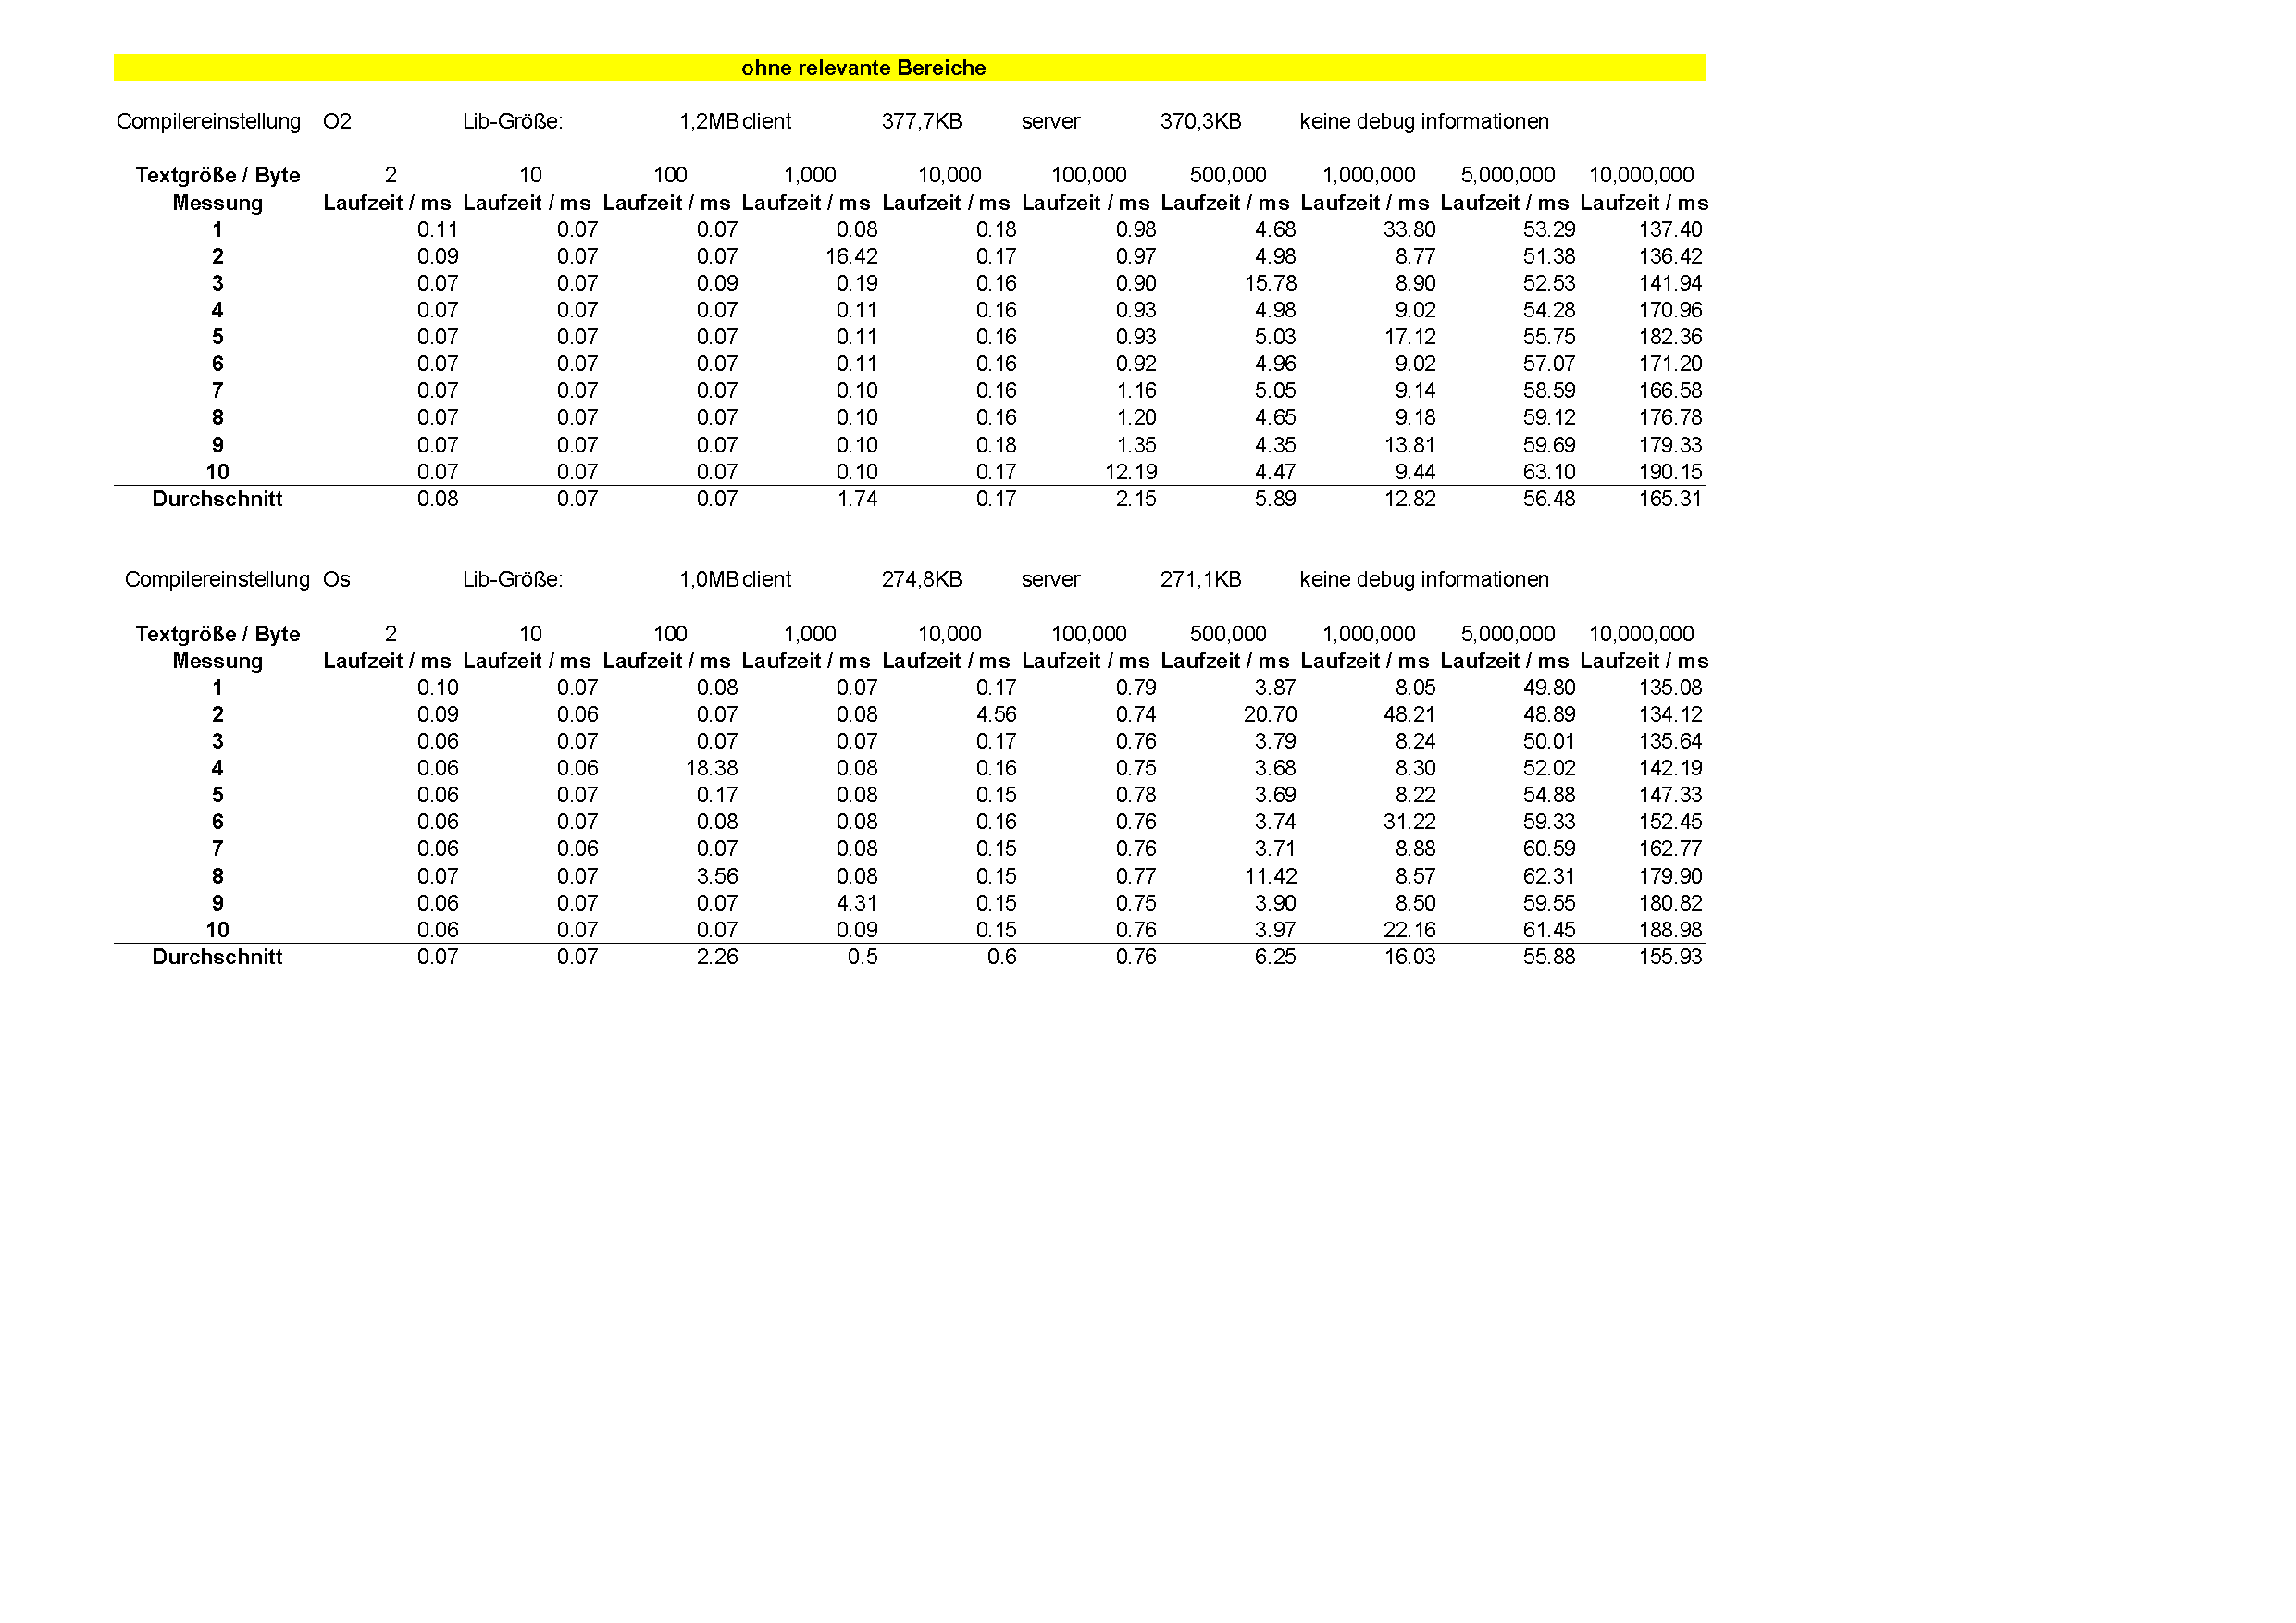
\includegraphics[angle=90,scale=.75]{MessungNormal_worp.pdf}
	\caption{Messung-Normal}	
\end{figure}

\newpage

\begin{figure}[H]
	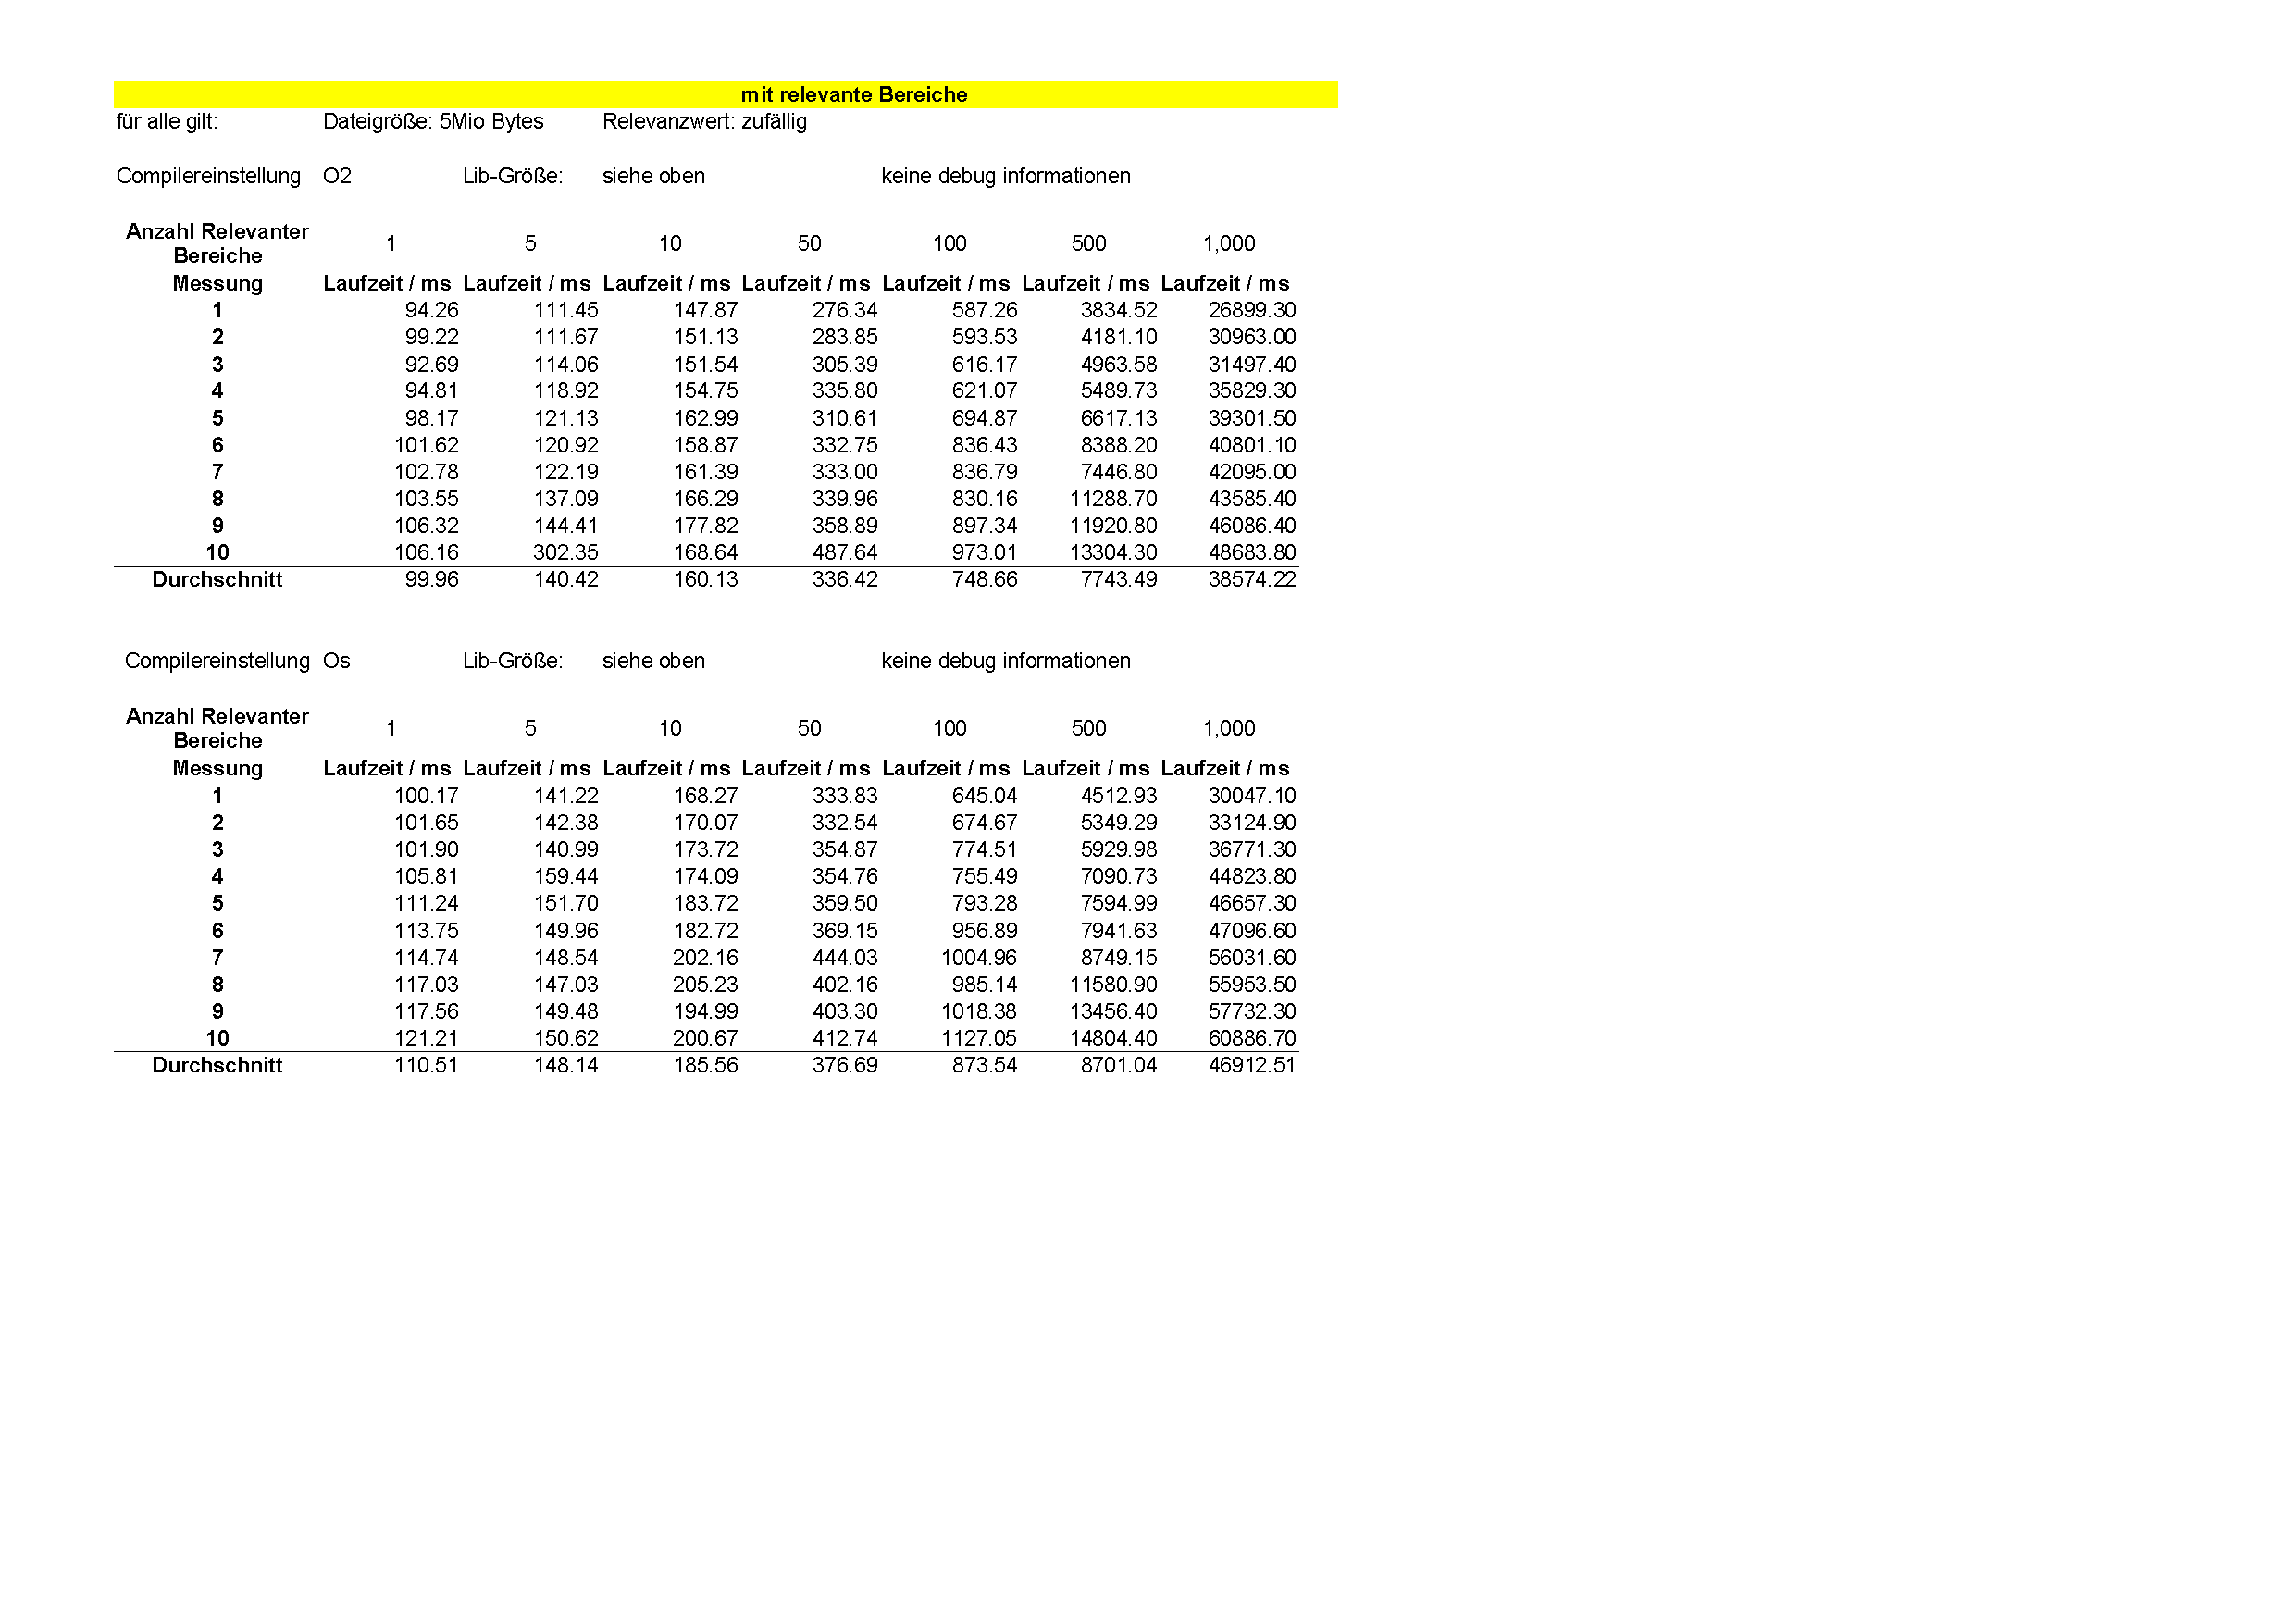
\includegraphics[angle=90,scale=.75]{MessungNormal_wrp.pdf}
	\caption{Messung-Normal}	
\end{figure}

\newpage

\begin{figure}[H]
	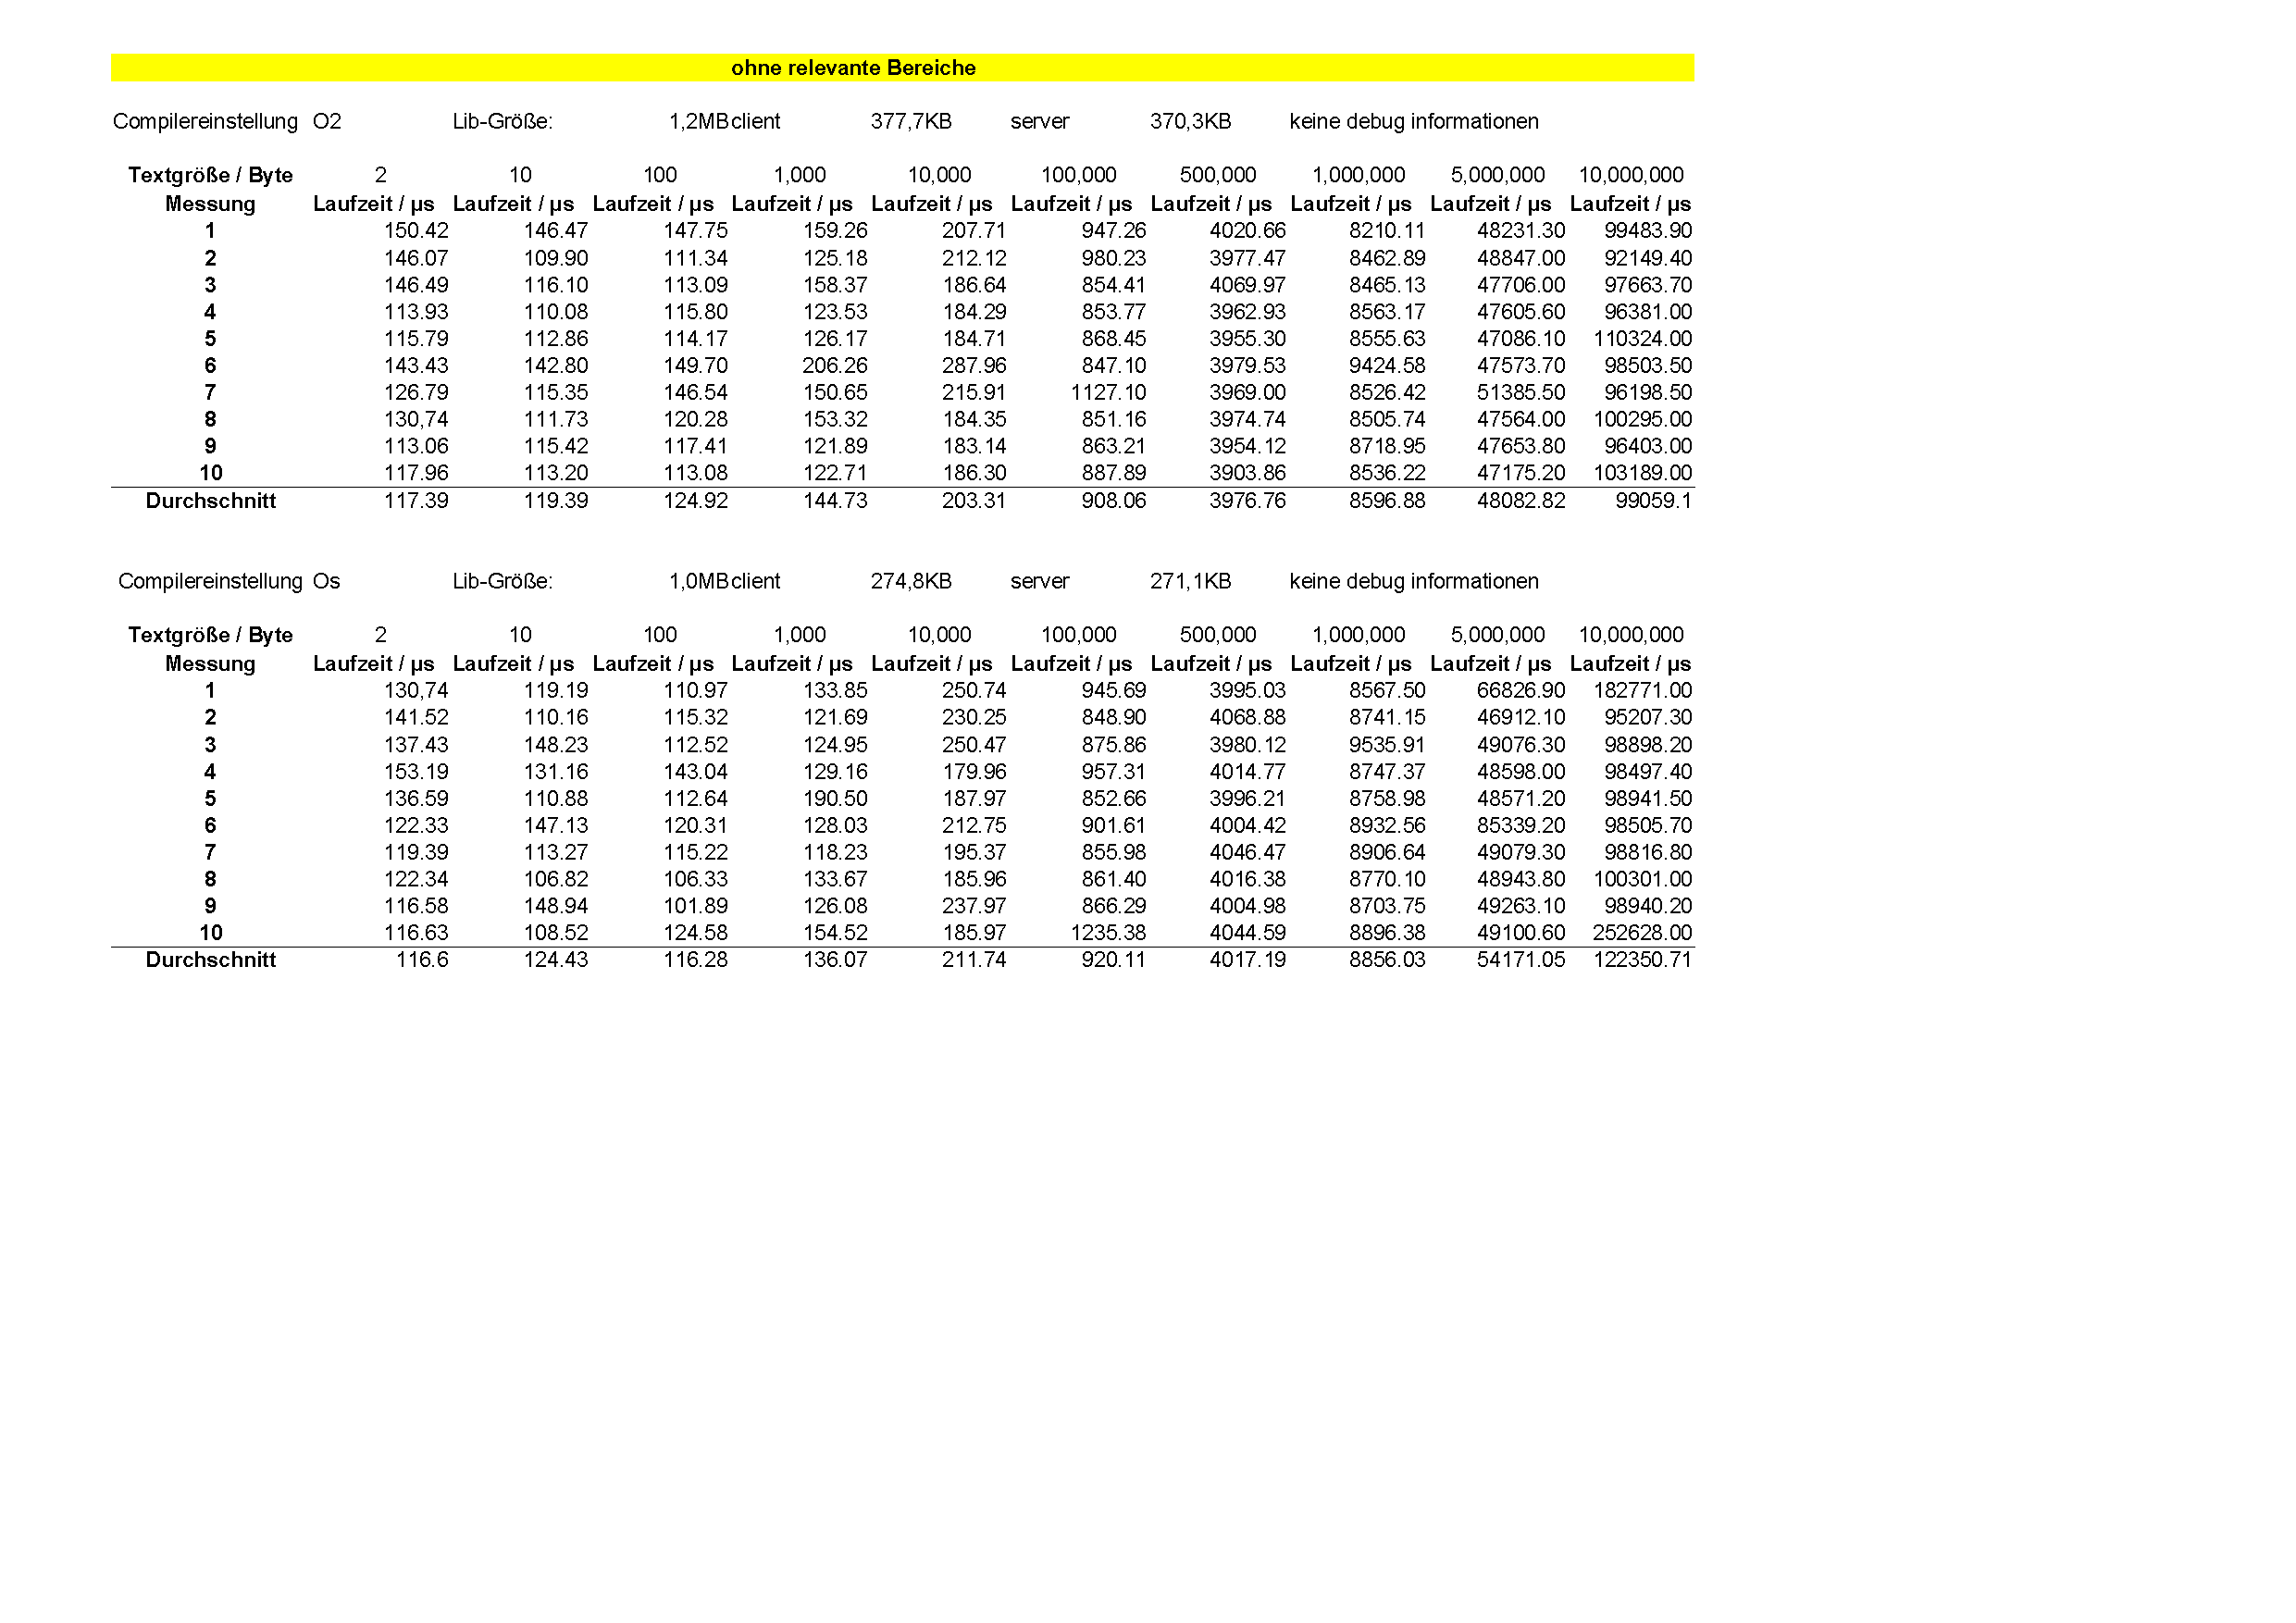
\includegraphics[angle=90,scale=.75]{MessungInitial_worp.pdf}
	\caption{Messung-Initial}	
\end{figure}

\newpage

\begin{figure}[H]
	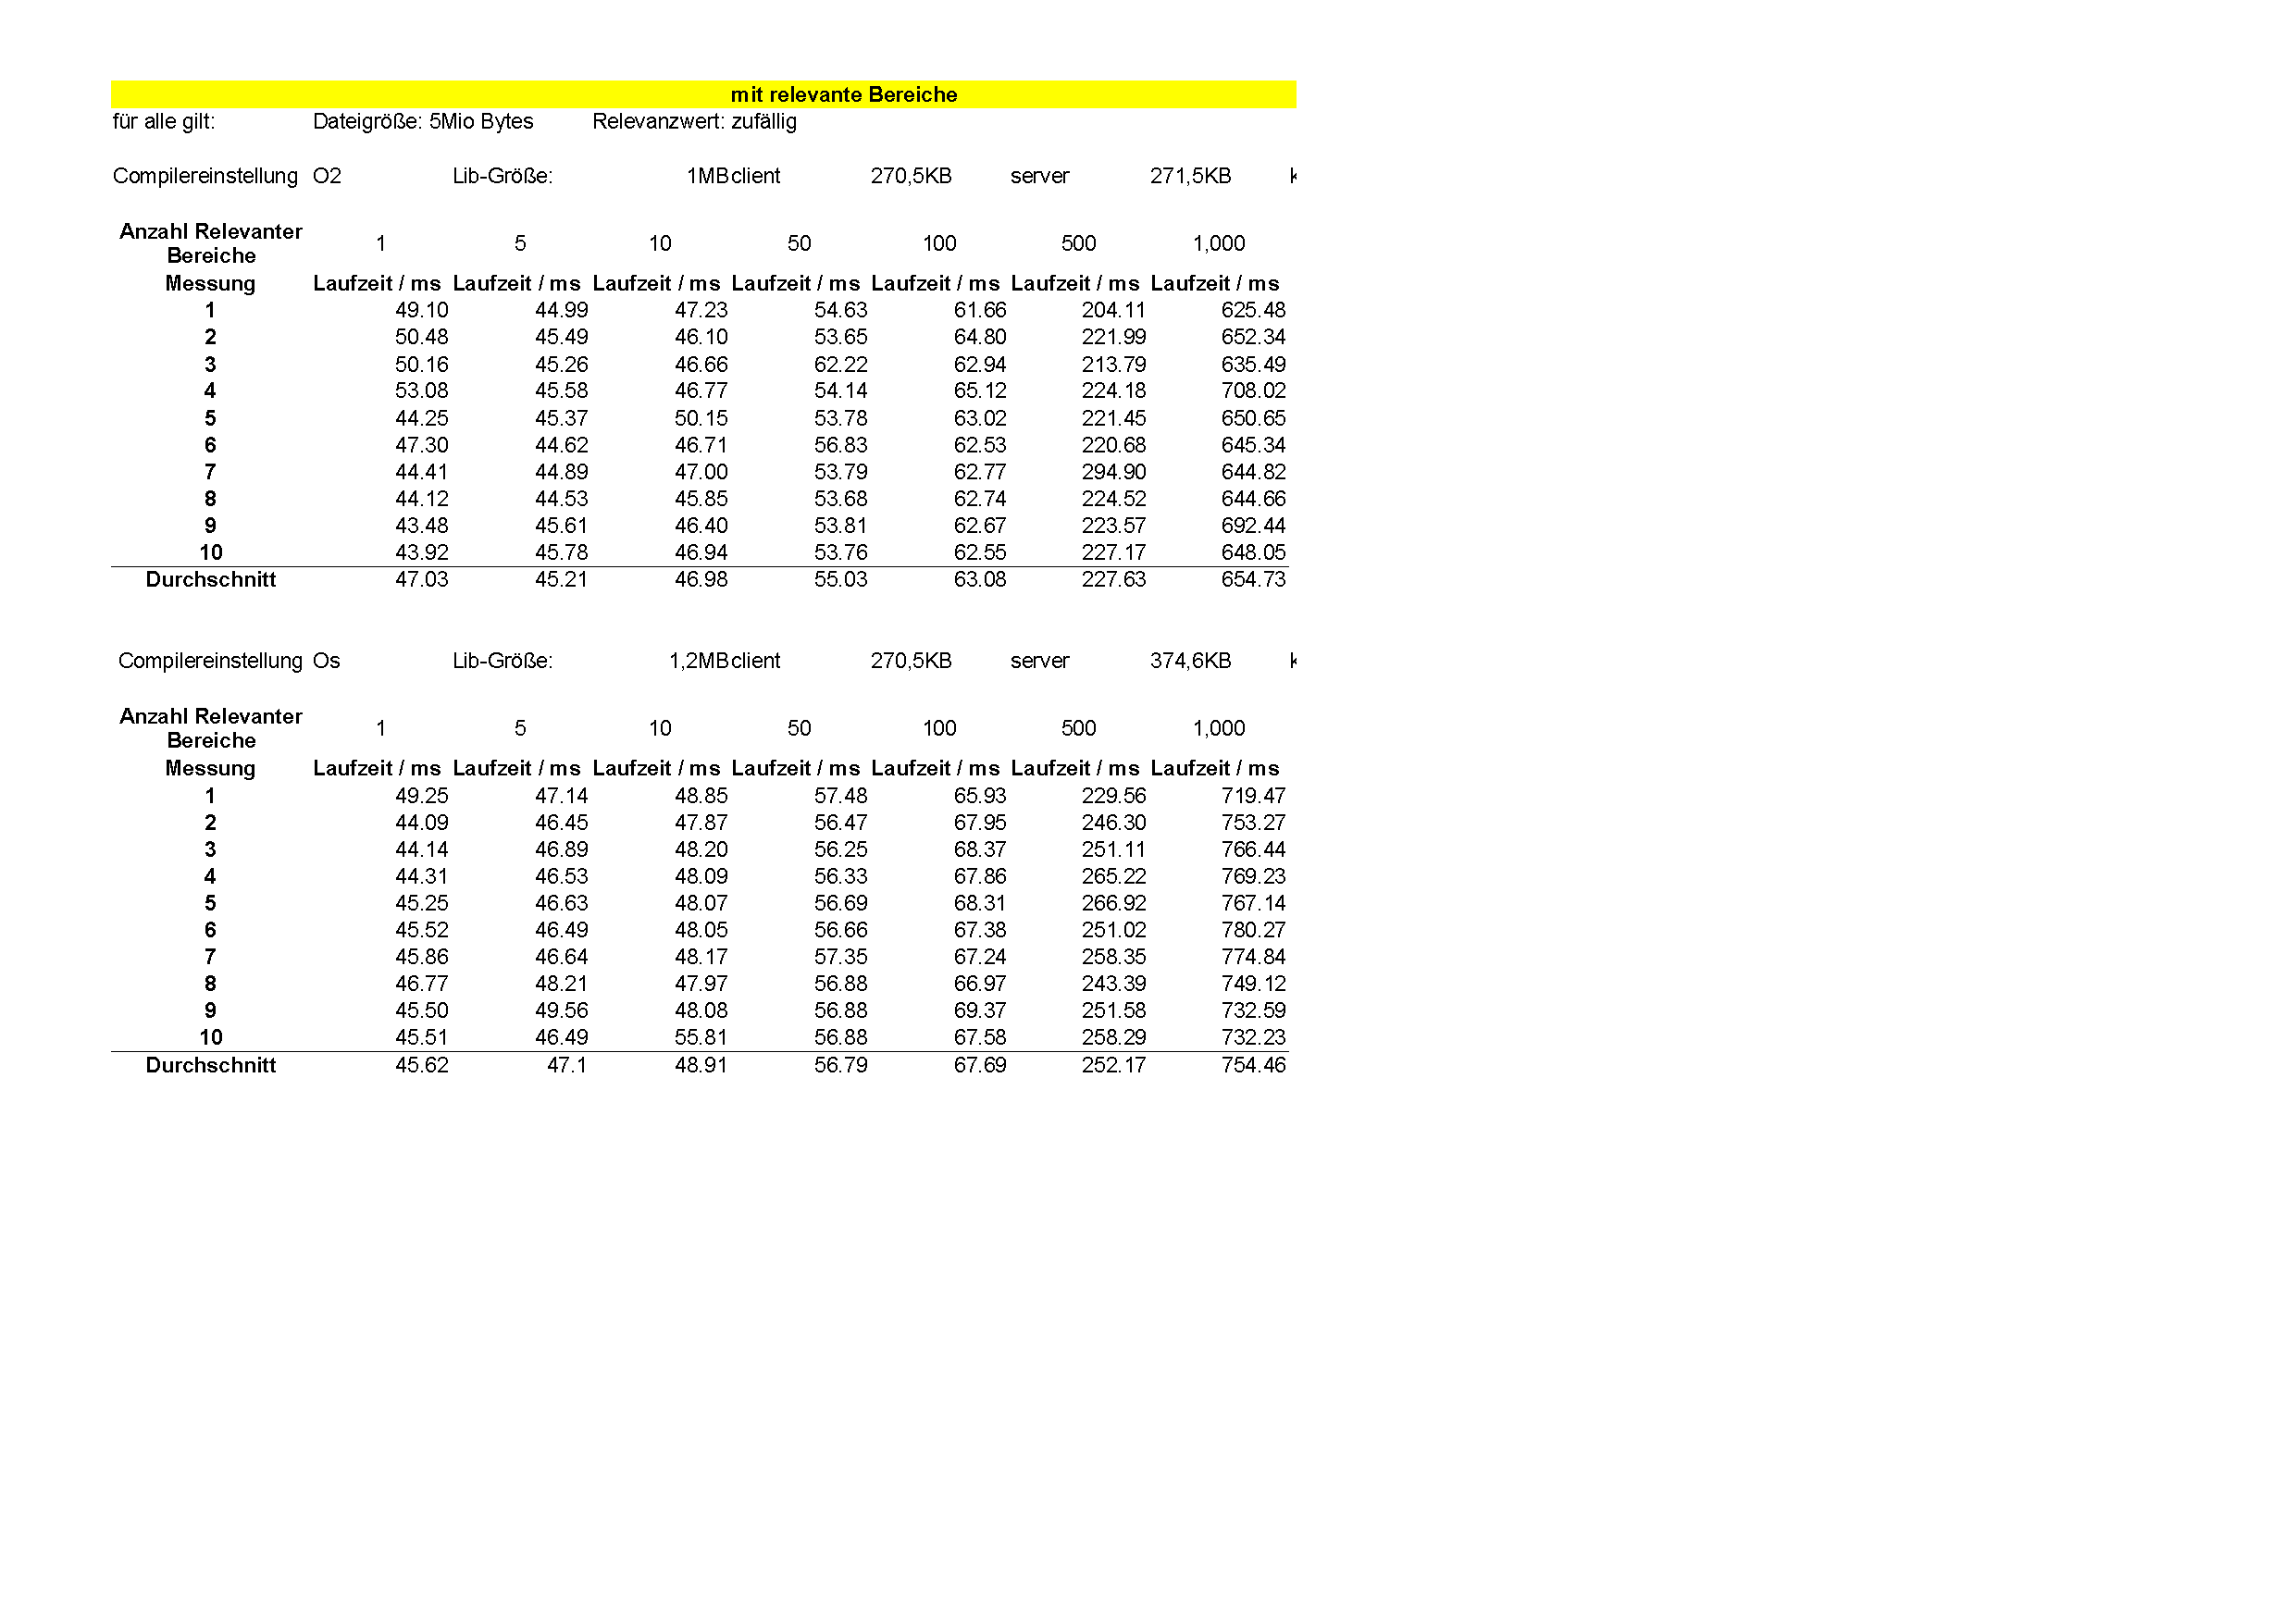
\includegraphics[angle=90,scale=.75]{MessungInitial_wrp.pdf}
	\caption{Messung-Initial}	
\end{figure}

% Die restlichen Diagramme. Müssen eventuell noch angepasst werden.

\newpage

\begin{figure}[H]
	\centering
	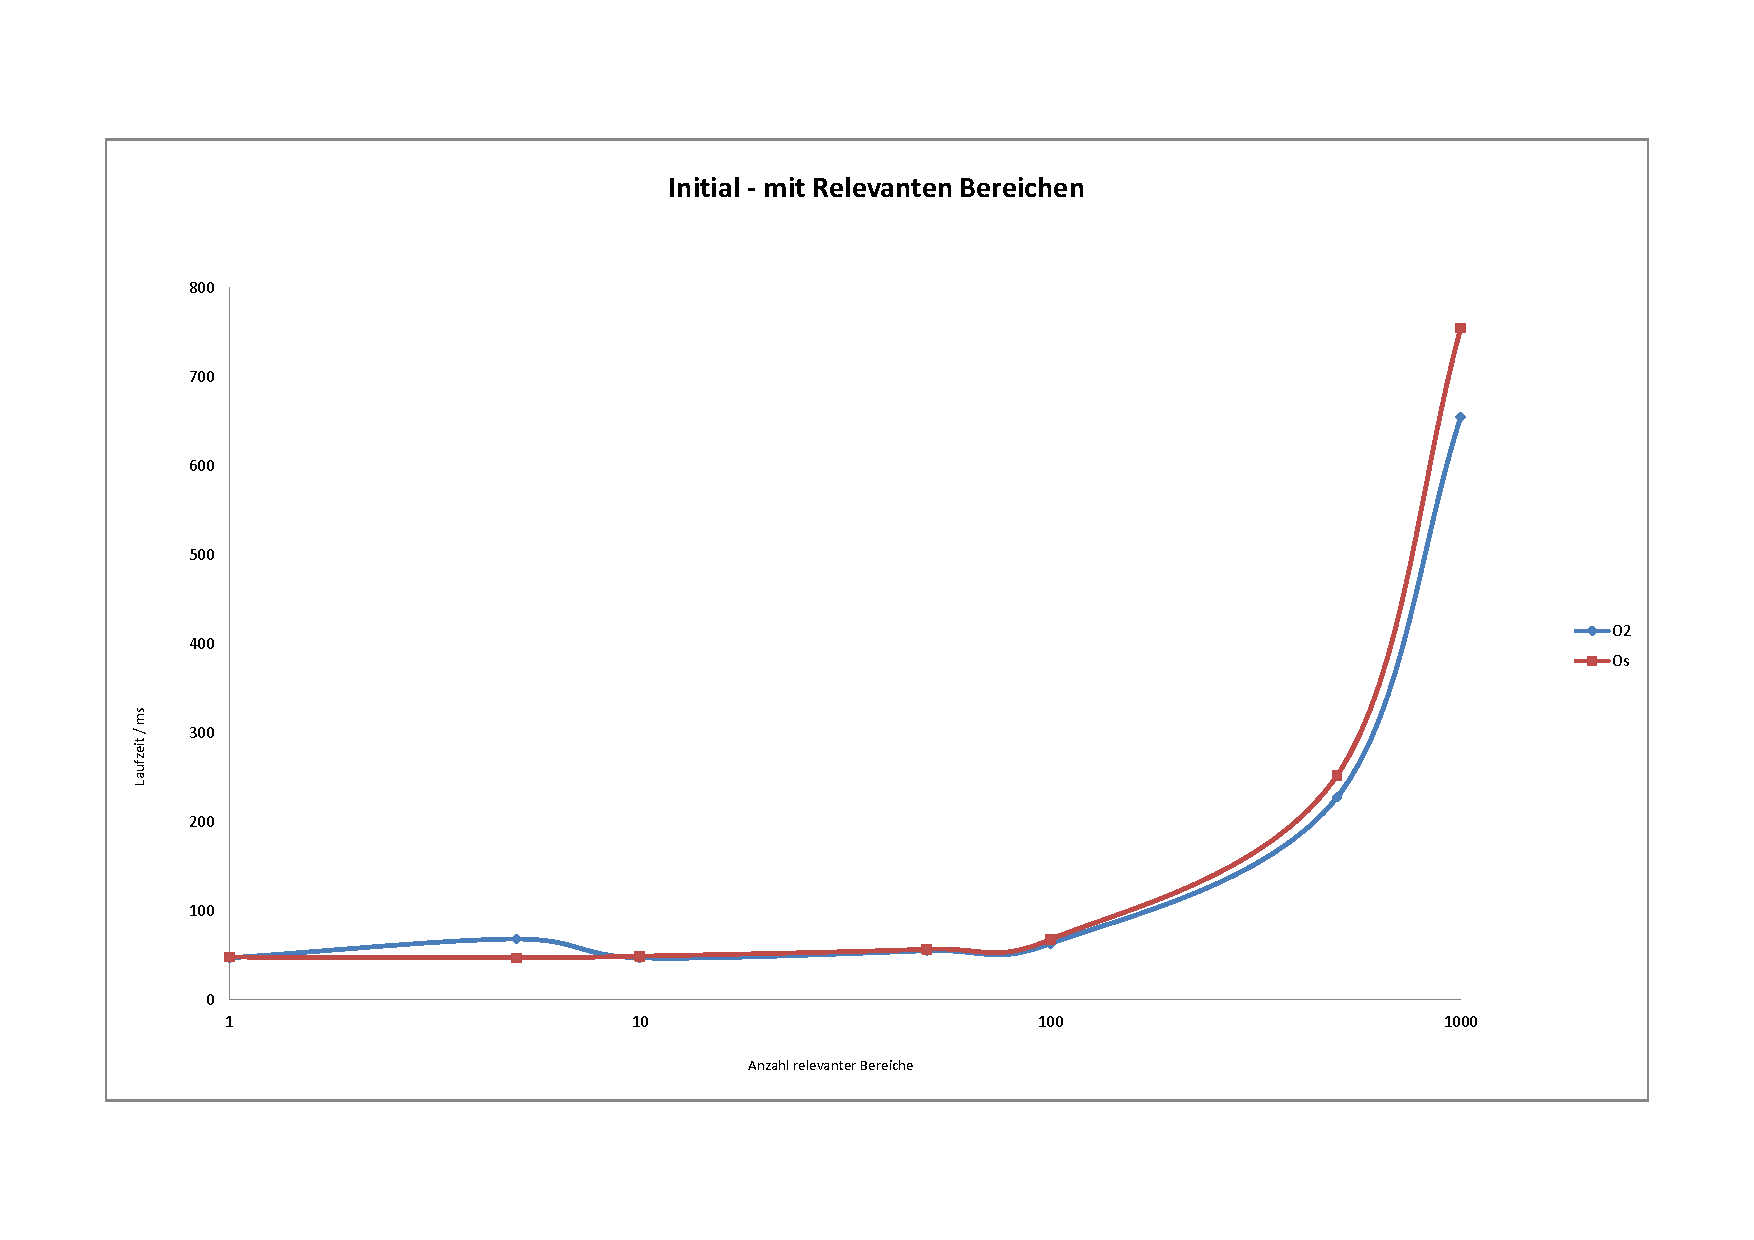
\includegraphics[angle=90,scale=.8]{DiagrammInitial_wrp.pdf}
	\label{fig:diagrammInitial_wrp}
	\caption{Messung-Initial mit relevanten Bereichen}
\end{figure}

\newpage

\begin{figure}[H]
	\centering
	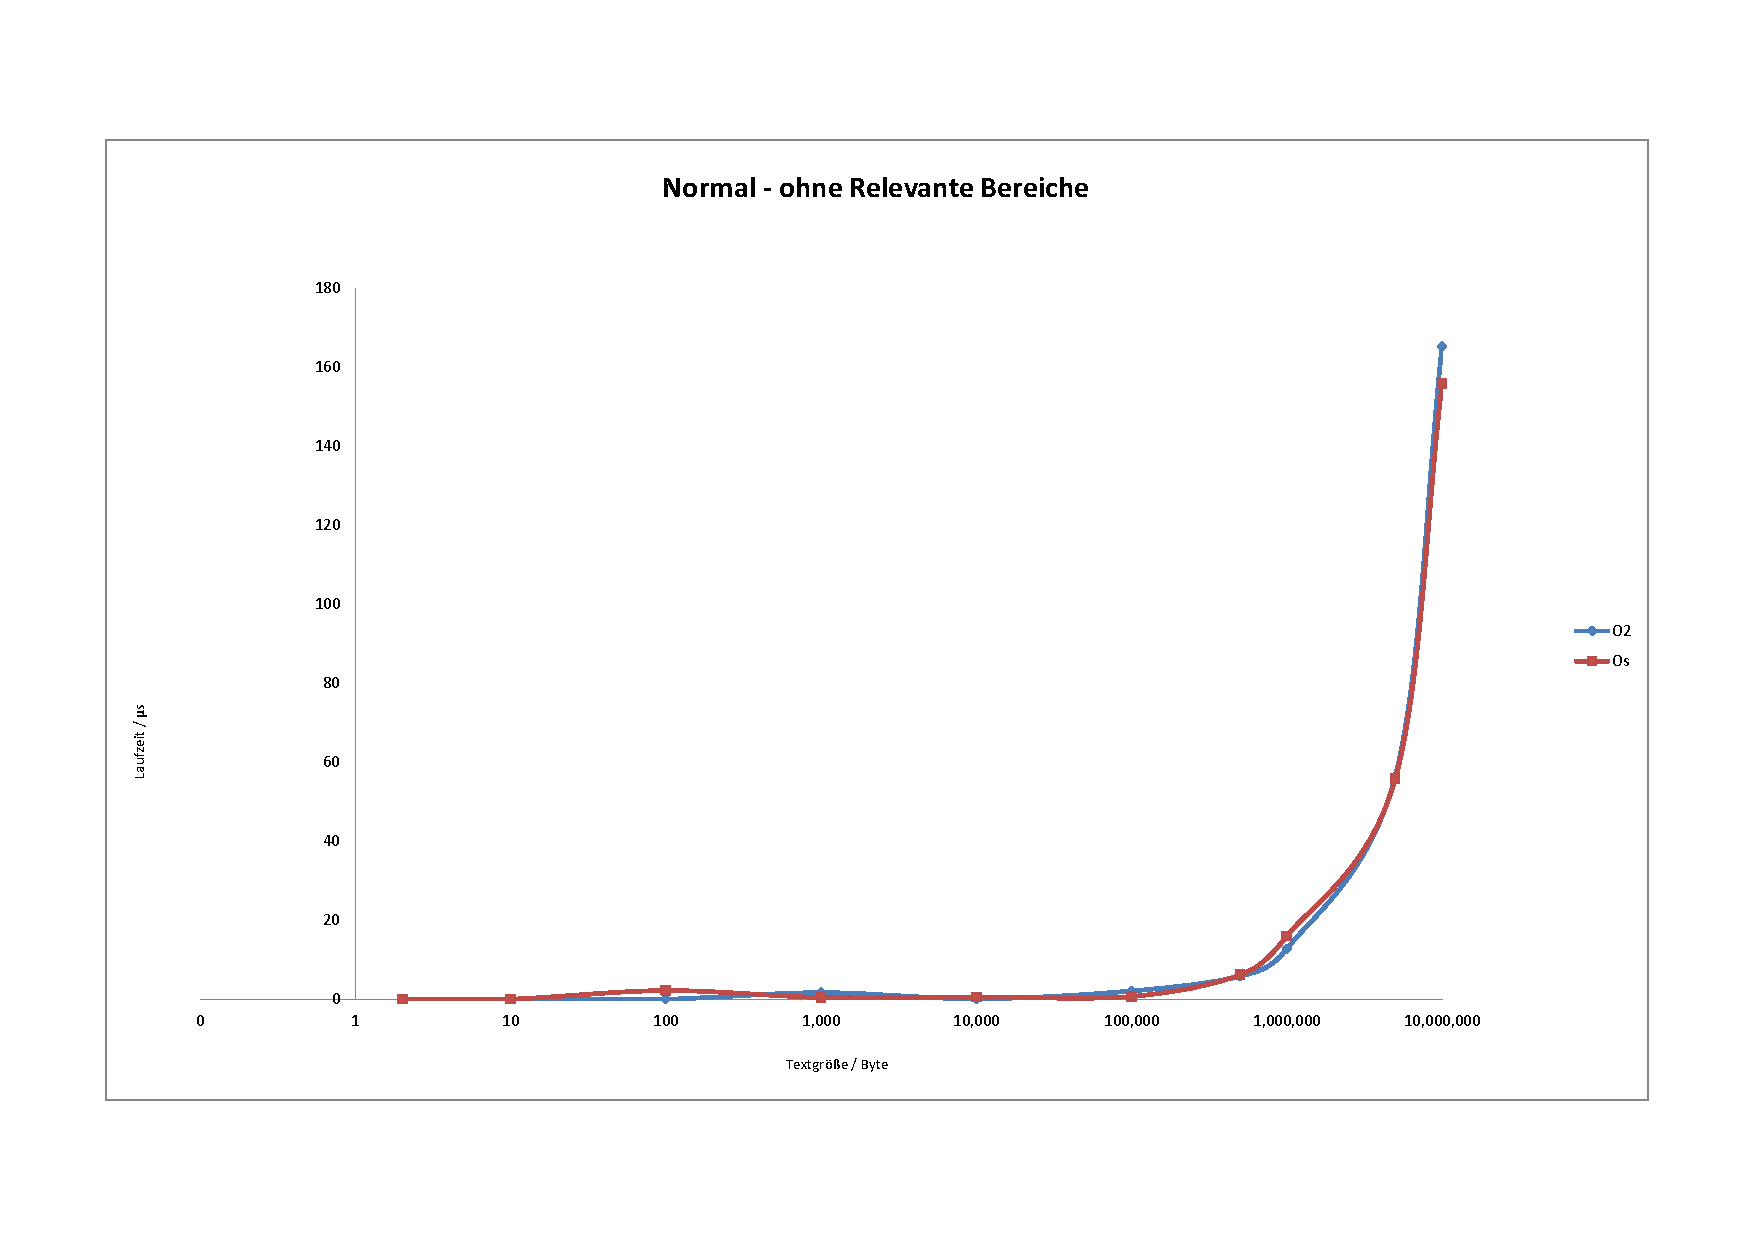
\includegraphics[angle=90,scale=.8]{DiagrammNormal_worp.pdf}
	\label{fig:diagrammNormal_worp}
	\caption{Messung-Normal ohne relevante Bereiche}
\end{figure}

\newpage

\begin{figure}[H]
	\centering
	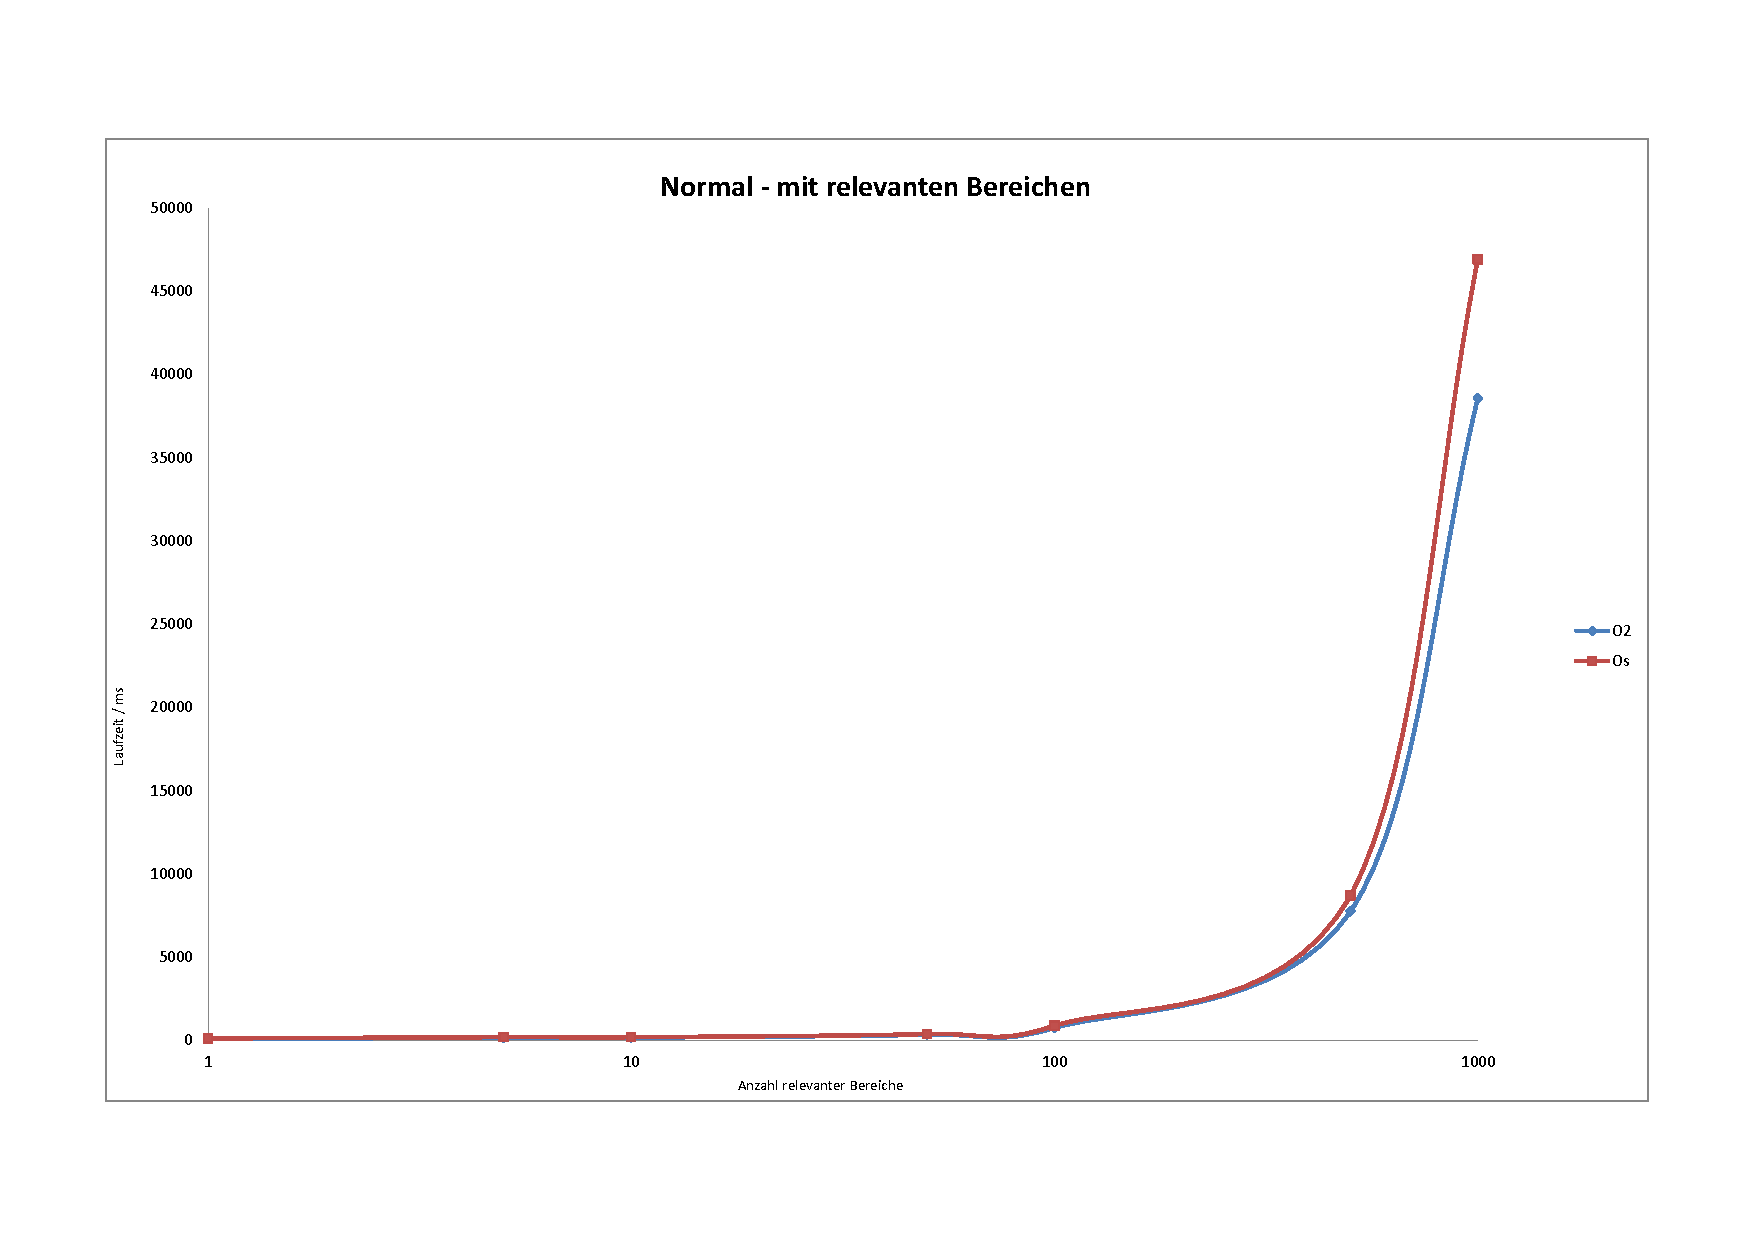
\includegraphics[angle=90,scale=.8]{DiagrammNormal_wrp.pdf}
	\label{fig:diagrammNormal_wrp}
	\caption{Messung-Normal mit relevanten Bereichen}
\end{figure}
